\documentclass[pdflatex,compress]{beamer}

%\usetheme[dark,framenumber,totalframenumber]{ElektroITK}
\usetheme[darktitle,framenumber,totalframenumber]{ElektroITK}
\usepackage{graphicx}
\usepackage{multicol}

\title{Data Communications}

\subtitle{Chapter 3 - Data Transmission}

\author{Mifta Nur Farid}

\date{8 March 2023}

\begin{document}

\maketitle

\begin{frame}
	\frametitle{Transmission Terminology}
	\begin{itemize}
		\item data transmission occurs between a transmitter \& receiver via some medium
		\item guided medium
		\begin{itemize}
			\item eg. twisted pair, coaxial cable, optical fiber
		\end{itemize}
		\item unguided / wireless medium
		\begin{itemize}
			\item eg. air, water, vacuum
		\end{itemize}
	\end{itemize}
\end{frame}

\begin{frame}{Transmission Terminology}
	\begin{itemize}
		\item direct link
		\begin{itemize}
			\item no intermediate devices
		\end{itemize}
		\item point-to-point
		\begin{itemize}
			\item direct link 
			\item only 2 devices share link
		\end{itemize}
		\item multi-point
		\begin{itemize}
			\item more than two devices share the link
		\end{itemize}
	\end{itemize}
\end{frame}

\begin{frame}{Transmission Terminology}
	\begin{itemize}
		\item simplex
		\begin{itemize}
			\item one direction
			\begin{itemize}
				\item eg. television
			\end{itemize}
		\end{itemize}
		\item half duplex
		\begin{itemize}
			\item either direction, but only one way at a time
			\begin{itemize}
				\item eg. police radio
			\end{itemize}
		\end{itemize}
		\item full duplex
		\begin{itemize}
			\item both directions at the same time
			\begin{itemize}
				\item eg. telephone
			\end{itemize}
		\end{itemize}
	\end{itemize}
\end{frame}

\begin{frame}
	\frametitle{Frequency, Spectrum and Bandwidth}
	\begin{itemize}
		\item time domain concepts
		\begin{itemize}
			\item analog signal
			\begin{itemize}
				\item various in a smooth way over time
			\end{itemize}
			\item digital signal
			\begin{itemize}
				\item maintains a constant level then changes to another constant level
			\end{itemize}
			\item periodic signal
			\begin{itemize}
				\item pattern repeated over time
			\end{itemize}
			\item aperiodic signal
			\begin{itemize}
				\item pattern not repeated over time
			\end{itemize}
		\end{itemize}
	\end{itemize}
\end{frame}

\begin{frame}
	\frametitle{Analog and Digital Signal}
	\begin{center}
		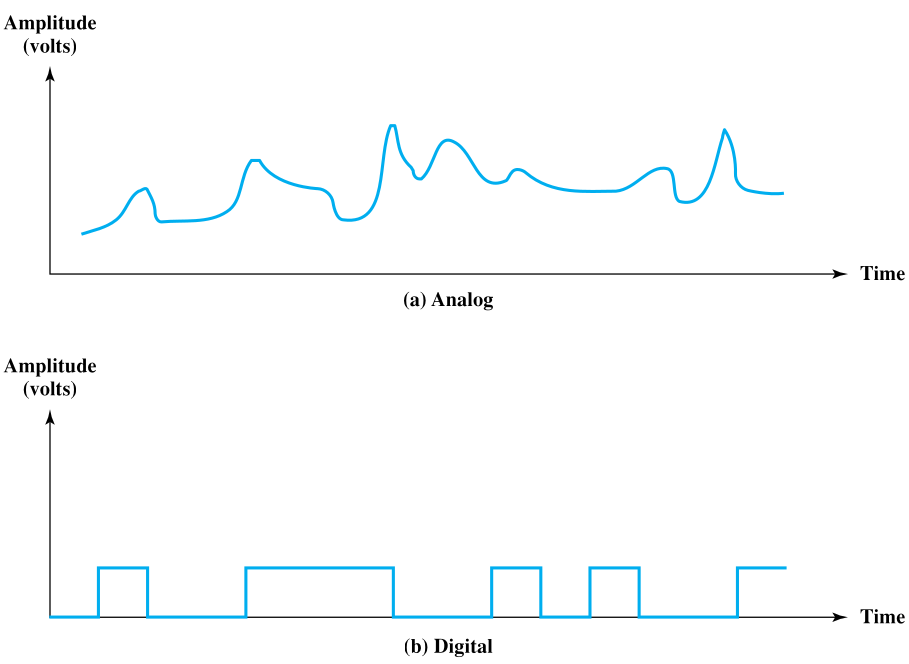
\includegraphics[width=0.8\linewidth]{img/img01}
	\end{center}
\end{frame}

\begin{frame}
	\frametitle{Periodic Signals}
	\begin{center}
		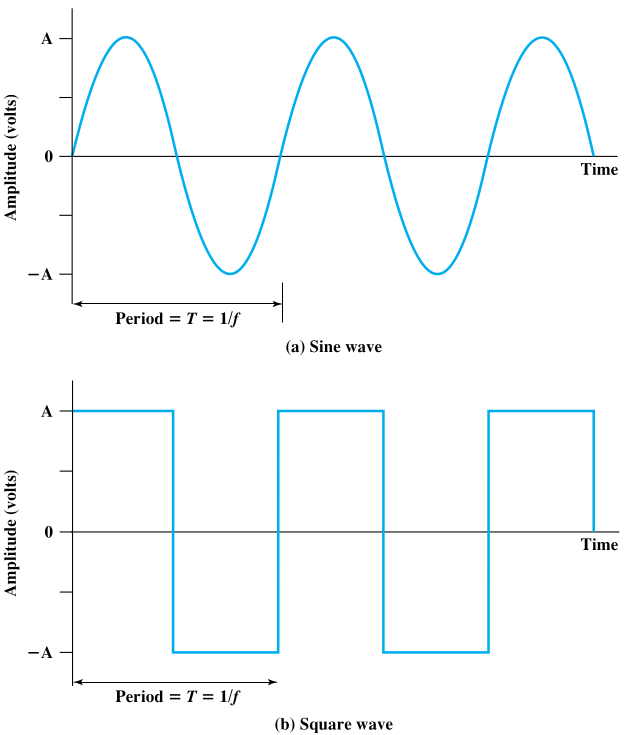
\includegraphics[height=0.9\textheight]{img/img02}
	\end{center}
\end{frame}

\begin{frame}
	\frametitle{Sine Wave}
	\begin{itemize}
		\item peak amplitude (A)
		\begin{itemize}
			\item maximum strength of signal
			\item volts
		\end{itemize}
		\item frequency (f)
		\begin{itemize}
			\item rate of change of signal
			\item Hertz (Hz) or cycles per second
			\item period = time for one repetition (T)
			\item T = 1/f
		\end{itemize}
		\item phase ($\phi$)
		\begin{itemize}
			\item relative position in time
		\end{itemize}
	\end{itemize}
\end{frame}

\begin{frame}
	\frametitle{Varying Sine Waves}
	\begin{equation*}
		s(t) = A \sin(2\pi ft + \phi)
	\end{equation*}
	\begin{center}
		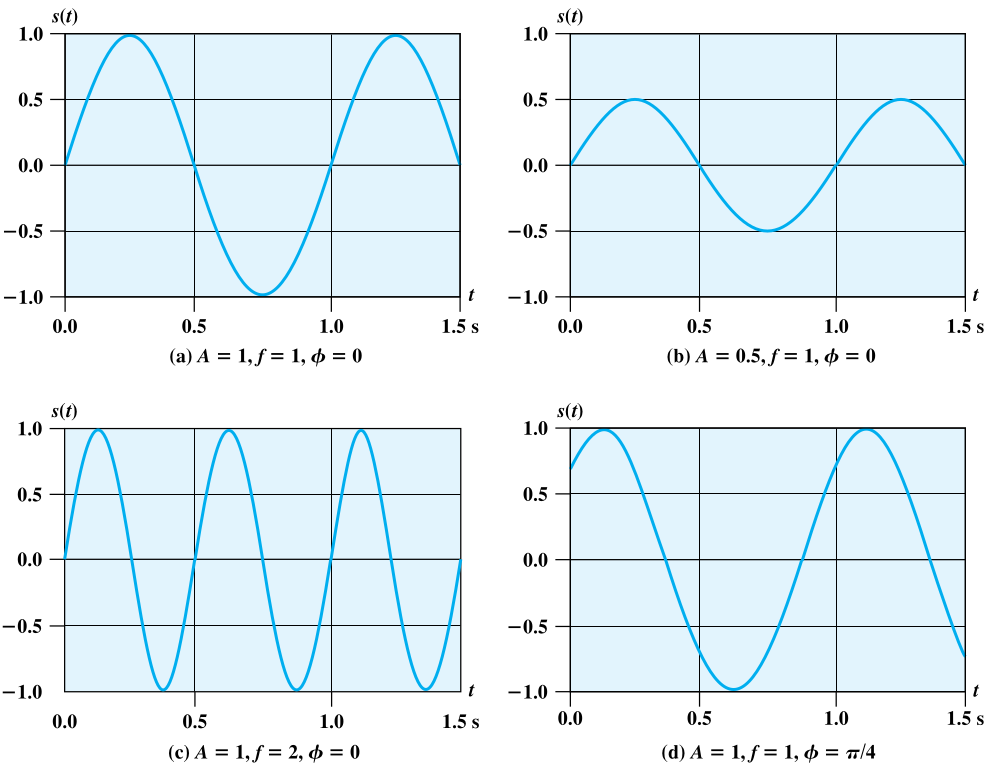
\includegraphics[height=0.72\textheight]{img/img03}
	\end{center}
\end{frame}

\begin{frame}
	\frametitle{Wavelength ($\lambda$)}
	\begin{itemize}
		\item is distance occupied by one cycle
		\item between two points of corresponding phase in two consecutive cycles
		\item assuming signal velocity v have $\lambda$ = vT
		\item or equivalently $\lambda$f = v
		\item especially when v = c
		\begin{itemize}
			\item c = 3 $\times$ 10$^\text{8}$ ms$^{-1}$ (speed of light in free space)
		\end{itemize}
	\end{itemize}
\end{frame}

\begin{frame}
	\frametitle{Frequency Domain Concepts}
	\begin{itemize}
		\item signal are made up of many frequencies
		\item components are sine waves
		\item Fourier analysis can shown that any signal is made up of component sine waves
		\item can plot frequency domain functions
	\end{itemize}
\end{frame}

\begin{frame}
	\frametitle{Addition of Frequency Components (T=1/f)}
	\begin{multicols}{2}
		\begin{center}
			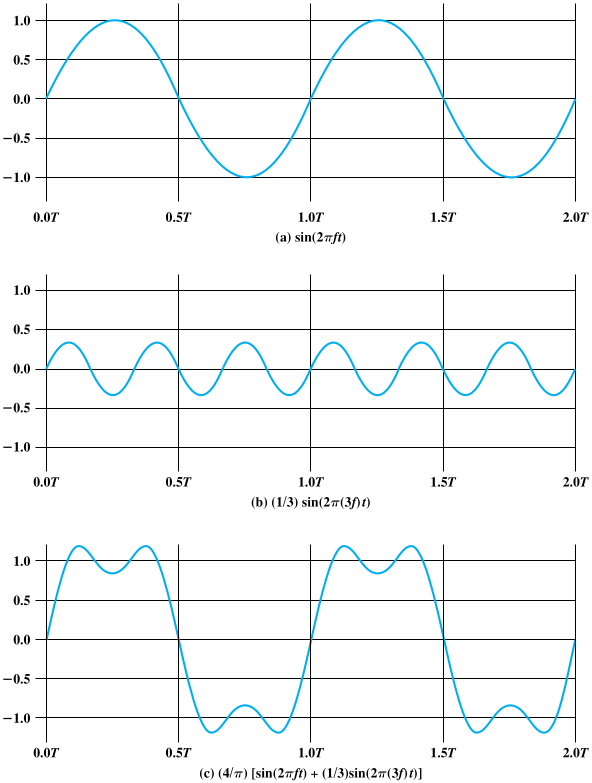
\includegraphics[height=0.85\textheight]{img/img04}
		\end{center}
		\columnbreak
		\begin{itemize}
			\item c is sum of f \& 3f
		\end{itemize}
	\end{multicols}
\end{frame}

\begin{frame}
	\frametitle{Frequency Domain Representations}
	\begin{center}
		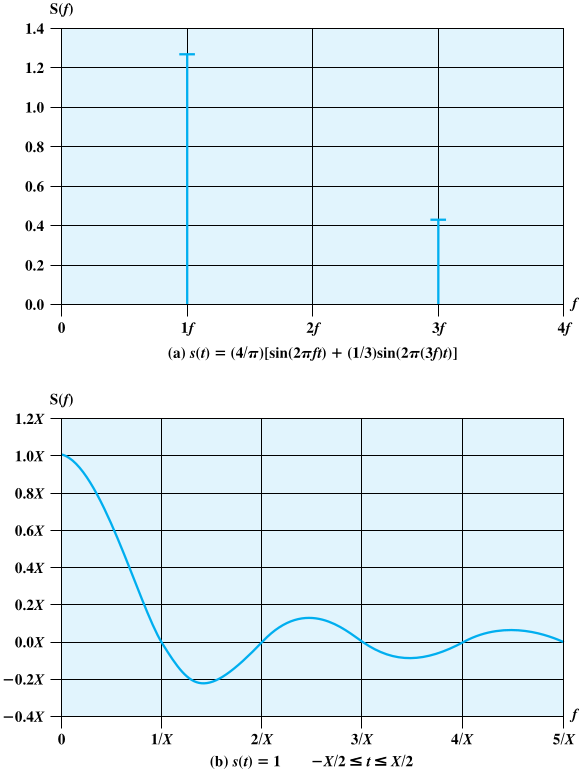
\includegraphics[height=0.85\textheight]{img/img05}
	\end{center}
\end{frame}

\begin{frame}
	\frametitle{Spectrum and Bandwidth}
	\begin{itemize}
		\item spectrum
		\begin{itemize}
			\item range of frequencies contained in signal
		\end{itemize}
		\item absolute bandwidth
		\begin{itemize}
			\item width of spectrum
		\end{itemize}
		\item effective bandwidth
		\begin{itemize}
			\item often just bandwidth
			\item narrow band of frequencies containing most energy
		\end{itemize}
		\item DC Component
		\begin{itemize}
			\item component of zero frequency
		\end{itemize}
	\end{itemize}
\end{frame}

\begin{frame}
	\frametitle{Data Rate and Bandwidth}
	\begin{itemize}
		\item any transmission system has a limited band of frequencies
		\item this limits the data rate that can be carried
		\item square have infinite components and hence bandwidth
		\item but most energy in first few components
		\item limited bandwidth increases distortion
		\item have a direct relationship between data rate \& bandwidth
	\end{itemize}
\end{frame}

\begin{frame}
	\frametitle{Analog and Digital Data Transmission}
	\begin{itemize}
		\item data 
		\begin{itemize}
			\item entities that convey meaning
		\end{itemize}
		\item signals \& signalling
		\begin{itemize}
			\item electric or electromagnetic representations of data, physically propagates along medium
		\end{itemize}
		\item transmission
		\begin{itemize}
			\item communication of data by propagation and processing of signals
		\end{itemize}
	\end{itemize}	
\end{frame}

\begin{frame}
	\frametitle{Acoustic Spectrum (Analog)}
	\begin{center}
		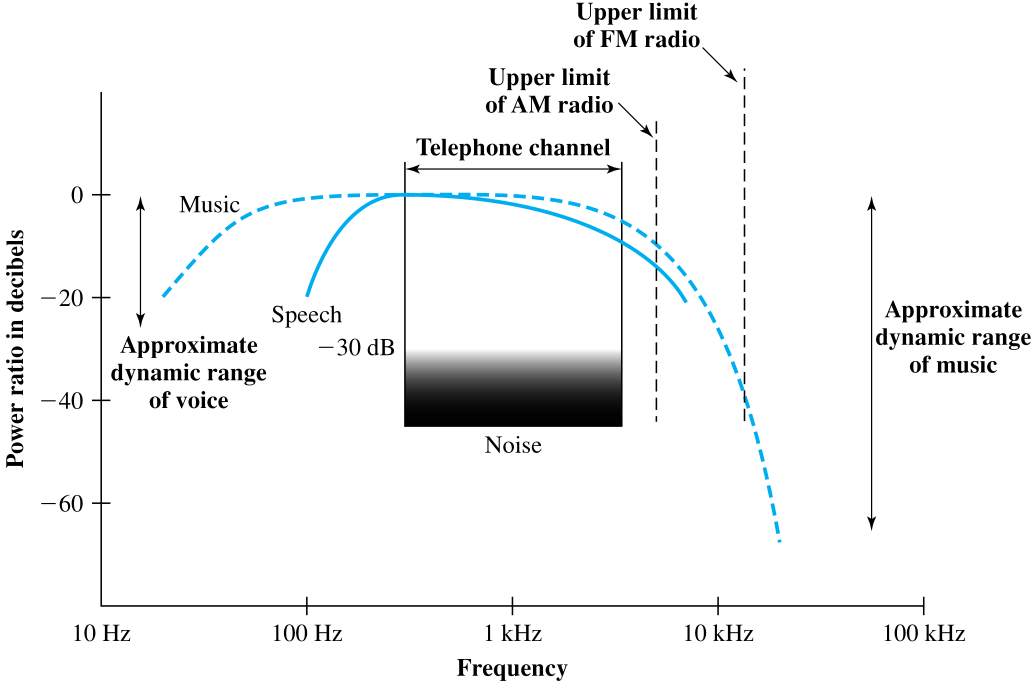
\includegraphics[height=0.9\textheight]{img/img06}
	\end{center}
\end{frame}

\begin{frame}
	\frametitle{Audio Signals}
	\begin{itemize}
		\item freq range 20Hz-20kHz (speech 100Hz-7kHz)
		\item easily converted into electromagnetic signals
		\item varying volume converted to varying voltage
		\item can limit frequency range for voice channel to 300-3400Hz
	\end{itemize}
	\begin{center}
		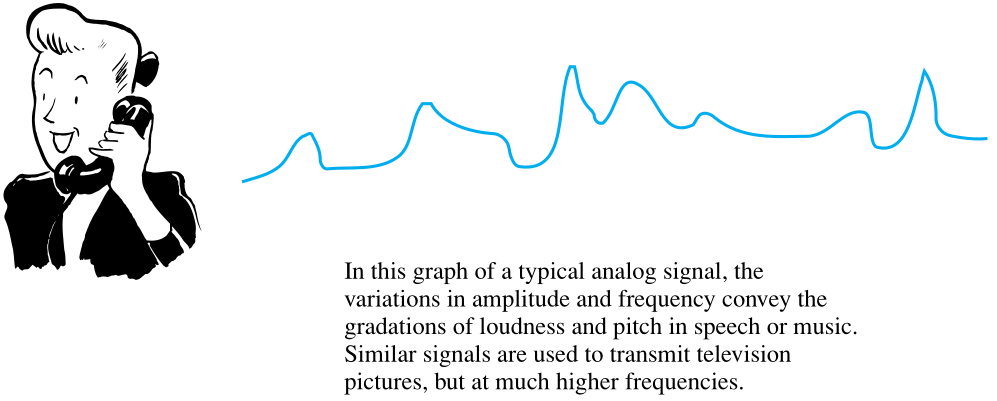
\includegraphics[width=\linewidth]{img/img07}
	\end{center}
\end{frame}

\begin{frame}
	\frametitle{Video Signals}
	\begin{itemize}
		\item USA - 483 lines per frame, at frames per sec
		\begin{itemize}
			\item have 525 lines but 42 lost during vertical retrace
		\end{itemize}
		\item 525 lines $\times$ 30 scans = 15750 lines per sec
		\begin{itemize}
			\item 63.5 $\mu$s per line
			\item 11 $\mu$s for retrace, so 52.5 $\mu$s per video line
		\end{itemize}
		\item max frequency if line alternates black and white
		\item horizontal resolution is about 450 lines giving 225 cycles of wave in 52.5 $\mu$s
		\item max frequency of 4.2MHz
	\end{itemize}
\end{frame}

\begin{frame}
	\frametitle{Digital Data}
	\begin{itemize}
		\item as generated by computers etc.
		\item has two dc components
		\item bandwidth depends on data rate
	\end{itemize}
	\begin{center}
		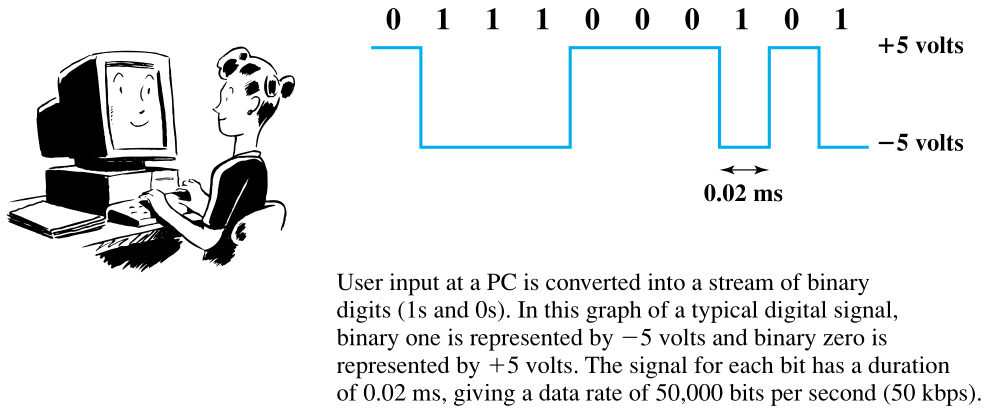
\includegraphics[width=\linewidth]{img/img08}
	\end{center}
\end{frame}

\begin{frame}
	\frametitle{Analog Signals}
	\begin{center}
		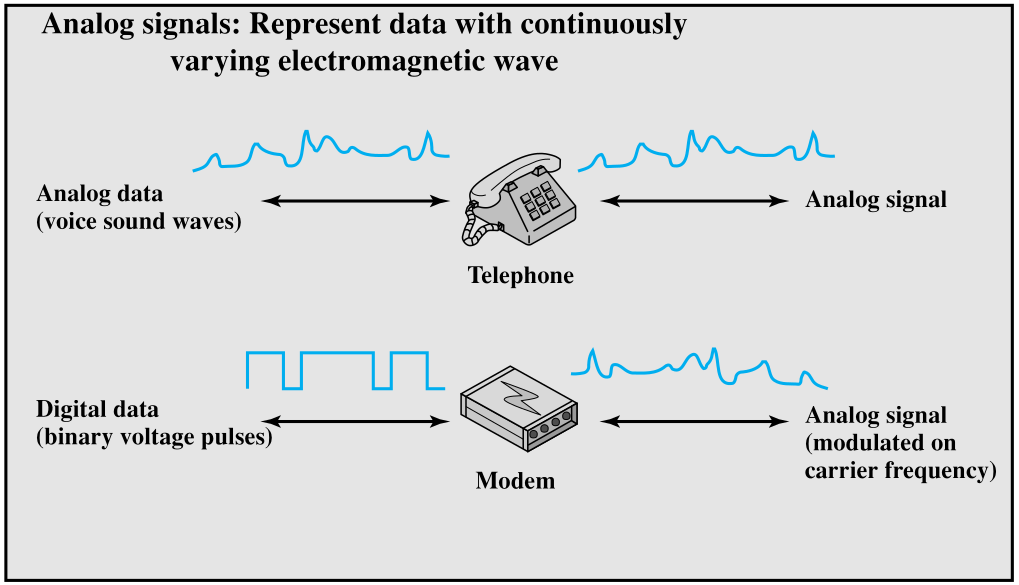
\includegraphics[width=\linewidth]{img/img09}
	\end{center}
\end{frame}

\begin{frame}
	\frametitle{Digital Signals}
	\begin{center}
		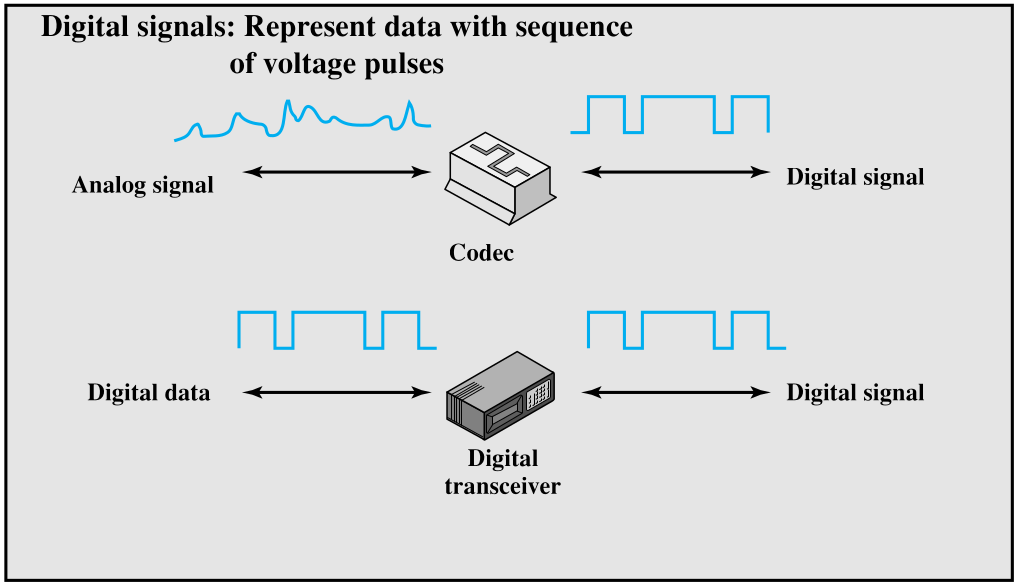
\includegraphics[width=\linewidth]{img/img10}
	\end{center}
\end{frame}

\begin{frame}
	\frametitle{Advantages and Disadvantages of Digital Signals}
	\begin{itemize}
		\item cheaper
		\item less susceptible to noise
		\item but greater attenuation
		\item digital now preferred choice
	\end{itemize}
	\begin{center}
		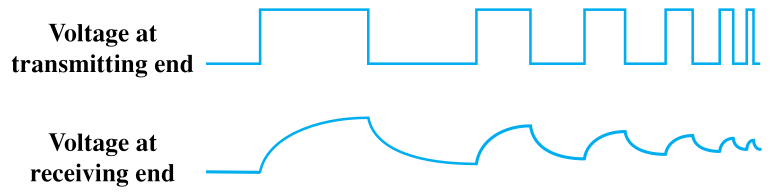
\includegraphics[width=\linewidth]{img/img11}
	\end{center}
\end{frame}

\begin{frame}
	\frametitle{Transmission Impairments}
	\begin{itemize}
		\item signal received may differ from signal transmitted causing:
		\begin{itemize}
			\item analog - degradation of signal quality
			\item digital - bit errors
		\end{itemize}
		\item most significant impairments are
		\begin{itemize}
			\item attenuation and attenuation distortion
			\item delay distortion
			\item noise
		\end{itemize}
	\end{itemize}
\end{frame}

\begin{frame}
	\frametitle{Attenuation}
	\begin{itemize}
		\item where signal strength falls off with distance
		\item depends on medium
		\item received signal strength must be:
		\begin{itemize}
			\item strong enough to be detected
			\item sufficiently higher than noise to receive without error
		\end{itemize}
		\item so increase strength using amplifiers/repeaters
		\item is also an increasing function of frequency
		\item so equalize attenuation across band of frequencies used
		\begin{itemize}
			\item eg. using loading coils or amplifiers
		\end{itemize}
	\end{itemize}
\end{frame}

\begin{frame}
	\frametitle{Delay Distortion}
	\begin{itemize}
		\item only occurs in guided media
		\item propagation velocity varies with frequency
		\item hence various frequency components arrive at different times
		\item particularly critical for digital data
		\item since parts of one bit spill over into others
		\item causing intersymbol interference
	\end{itemize}
\end{frame}

\begin{frame}
	\frametitle{Noise}
	\begin{itemize}
		\item additional signals inserted between transmitter and receiver
		\item thermal
		\begin{itemize}
			\item due to thermal agitation of electrons
			\item uniformly distributed
			\item white noise
		\end{itemize}
		\item intermodulation
		\begin{itemize}
			\item signals that are the sum and difference of original frequencies sharing a medium
		\end{itemize}
	\end{itemize}
\end{frame}

\begin{frame}{Noise}
	\begin{itemize}
		\item crosstalk
		\begin{itemize}
			\item a signal from one line is picked up by another
		\end{itemize}
		\item impulse
		\begin{itemize}
			\item irregular pulses or spikes
			\begin{itemize}
				\item eg. external electromagnetic interference
			\end{itemize}
			\item short duration
			\item high amplitude
			\item a minor annoyance for analog signals
			\item but a major source of error in digital data
			\begin{itemize}
				\item a noise spike could corrupt many bits
			\end{itemize}
		\end{itemize}
	\end{itemize}
\end{frame}

\begin{frame}
	\frametitle{Channel Capacity}
	\begin{itemize}
		\item max possible data rate on comms channel 
		\item is a function of
		\begin{itemize}
			\item data rate - in bits per second
			\item bandwidth - in cycles per second or Hertz
			\item noise - on comms link
			\item error rate - of corrupted bits
		\end{itemize}
		\item limitations due to physical properties
		\item want most efficient use of capacity
	\end{itemize}
\end{frame}

\begin{frame}
	\frametitle{Nyquist Bandwidth}
	\begin{itemize}
		\item consider noise free channels
		\item if rate of signal transmission is 2B then can carry signal with frequencies no greater than B 
		\begin{itemize}
			\item ie. given bandwidth B, highest signal rate is 2B
		\end{itemize}
		\item for binary signals, 2B bps needs bandwidth B Hz
		\item can increase rate by using M signal levels
		\item Nyquist Formula is: C = 2B $\log_2$M
		\item so increase rate by increasing signals
		\begin{itemize}
			\item at cost of receiver complexity
			\item limited by noise \& other impairments
		\end{itemize}
	\end{itemize}
\end{frame}

\begin{frame}
	\frametitle{Shannon Capacity Formula}
	\begin{itemize}
		\item consider relation of data rate, noise \& error rate
		\begin{itemize}
			\item faster data rate shortens each bit so bursts of noise affects more bits
			\item given noise level, higher rates means higher errors
		\end{itemize}
		\item Shannon developed formula relating these to signal to noise ratio (in decibels)
		\item $\text{SNR}_{\text{db}}$ = 10 $\log_{10}$ (signal/noise)
		\item Capacity C = B $\log_2$(1+SNR)
		\begin{itemize}
			\item theoretical maximum capacity
			\item get lower in practise
		\end{itemize}
	\end{itemize}
\end{frame}

\begin{frame}
	\frametitle{Summary}
	\begin{itemize}
		\item looked at data transmission issues
		\item frequency, spectrum \& bandwidth
		\item analog vs digital signals
		\item transmission impairments
	\end{itemize}
\end{frame}

\end{document}
